% !TeX spellcheck = en_US
\documentclass[12pt,aspectratio=169]{beamer}

\usetheme[progressbar=frametitle]{metropolis}
\usepackage{appendixnumberbeamer}

\usepackage{booktabs}
\usepackage[scale=2]{ccicons}

\usepackage{pgfplots}
\usepgfplotslibrary{dateplot}

\usepackage{xspace}
\newcommand{\themename}{\textbf{\textsc{metropolis}}\xspace}

\usepackage{verbatim}

\usepackage[acronym]{glossaries}
\glsdisablehyper
\makeglossaries
\newacronym{sdn}{SDN}{Software Defined Networking}

\title{Adaptive network slicing}
\subtitle{Project course}
\date{13. 01. 2020.}
\author{M\'at\'e Eckl\\\small{Supervisor: Prof. Fabrizio Granelli}}
\institute{Università di Trento\\Department of Information Engineering and Computer Science}
% \titlegraphic{\hfill\includegraphics[height=1.5cm]{logo.pdf}}

\begin{document}

\maketitle

% Target audience: The supervisor
% Style: To the point, not too academic

\begin{comment}
% template
\begin{frame}[label=]{}
	\begin{itemize}
	\end{itemize}
\end{frame}
\end{comment}


\section{Design}
\begin{frame}[label=goal]{Goal}
	\begin{itemize}
		\item Assign resources to different flows
		\item Reuse unused resources adaptively
	\end{itemize}
\end{frame}

\begin{frame}[label=slicing-possibilities]{Slicing possibilities}
	\begin{itemize}
		\item Solutions for slicing specifically
		\begin{itemize}
			\item Flowvisor
			\item Delftvisor
			\item FlowSpace firewall
			\item Either obsolete or too experimental
			\item Or do not implement flow-based slicing
		\end{itemize}
		\item General SDN controllers
		\begin{itemize}
			\item No multi-tenant support
			\item Actively developed
			\item Support for newer OpenFlow versions
		\end{itemize}
	\end{itemize}
\end{frame}

\begin{frame}[label=slicing-tech-selection]{Slicing technology selection -- The RYU controller}
	\begin{itemize}
		\item Supports OpenFlow1.3 -- \\Convenient capabilities for QoS setting
		\item Well developed
		\item Optimal for prototyping
	\end{itemize}
	\begin{tikzpicture}[overlay,remember picture]
	\node[anchor=south east,xshift=200pt,yshift=-60pt]
	at (current page) {
		
\includegraphics[width=0.4\linewidth]{resources/ryu-logo.png}
	};
	\end{tikzpicture}
\end{frame}

\begin{frame}[label=controller-implementation]{Controller implementation}
	\begin{itemize}
		\item Pseudo network slicing -- Flow-based QoS
		\item OpenFlow 1.3
		\item 2 built in applications -- REST API interface handlers
		\item 2 custom
		\begin{itemize}
			\item QoS Switch -- Basic switch that respects QoS
			\item \textbf{Adapting monitor} -- Set, monitor and adapt QoS settings
		\end{itemize}
	\end{itemize}
\end{frame}

\begin{frame}[label=adapting-monitor]{Adapting monitor implementation -- monitoring}
	\begin{itemize}
		\item Monitor matching to different flows
		\item OFPFlowStats.byte\_count: matched number of bytes
	\end{itemize}
	\bigskip
	\begin{equation*}
		Avg [\text{Bps}] = \frac{\text{byte\_count}(t_0) - \text{byte\_count}(t_{-(\text{window size}-1)})}{\text{window size}-1} \cdot \frac{1}{\Delta t} \bigg|_{\Delta t = 5s\text{; window size}=10}
	\end{equation*}
\end{frame}

\begin{frame}[label=flow-adaptation]{Adapting monitor implementation -- flow adaptation}
	\centering
	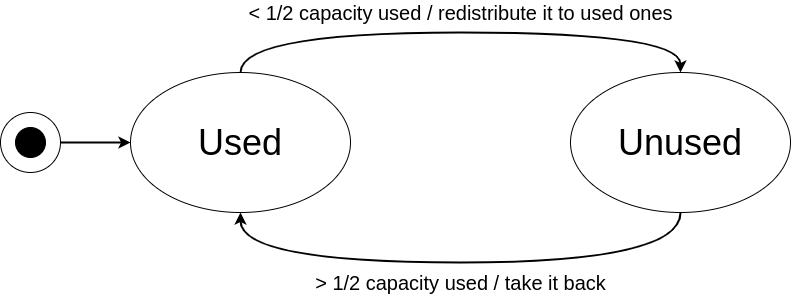
\includegraphics[width=\linewidth]{resources/flow-states.png}
\end{frame}


\section{Demo}

\begin{frame}[label=demo-environment]{Demo environment}
	\centering
	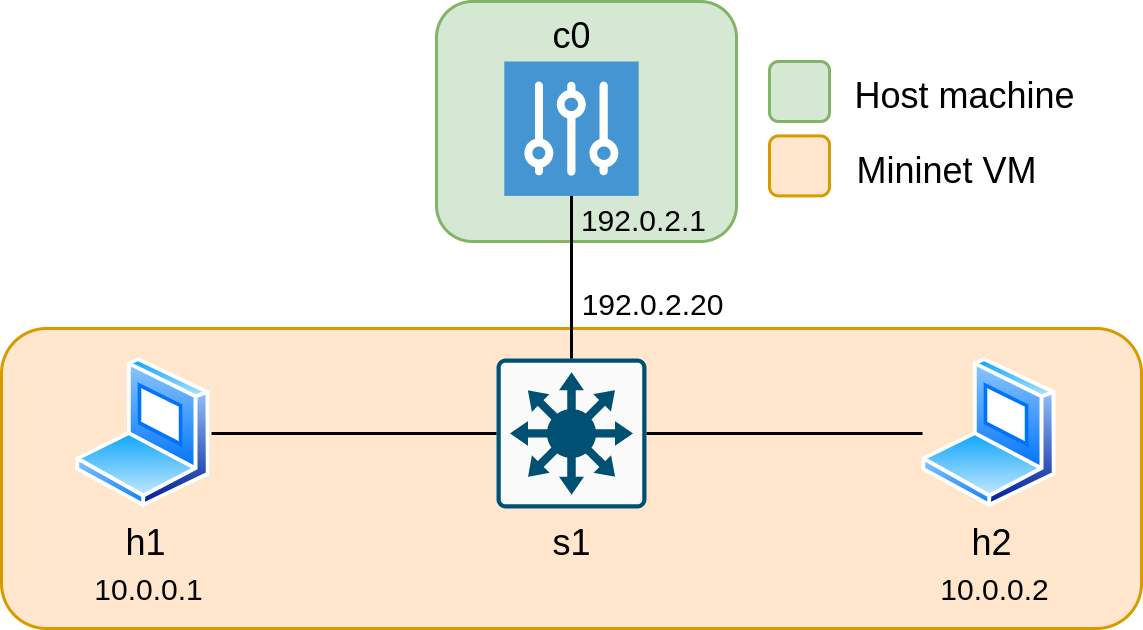
\includegraphics[width=0.9\linewidth]{resources/topology.png}
\end{frame}

\begin{frame}[label=demo-flows]{Demo flows}
	\centering
	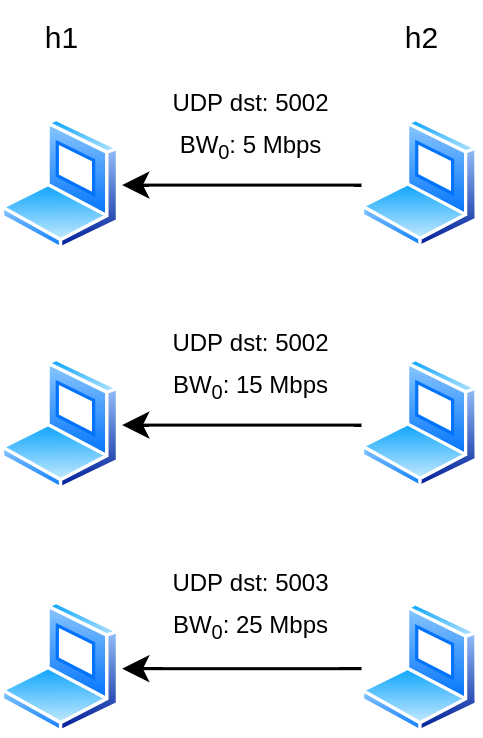
\includegraphics[width=0.25\linewidth]{resources/flow-definitions.png}\hspace{10mm}
	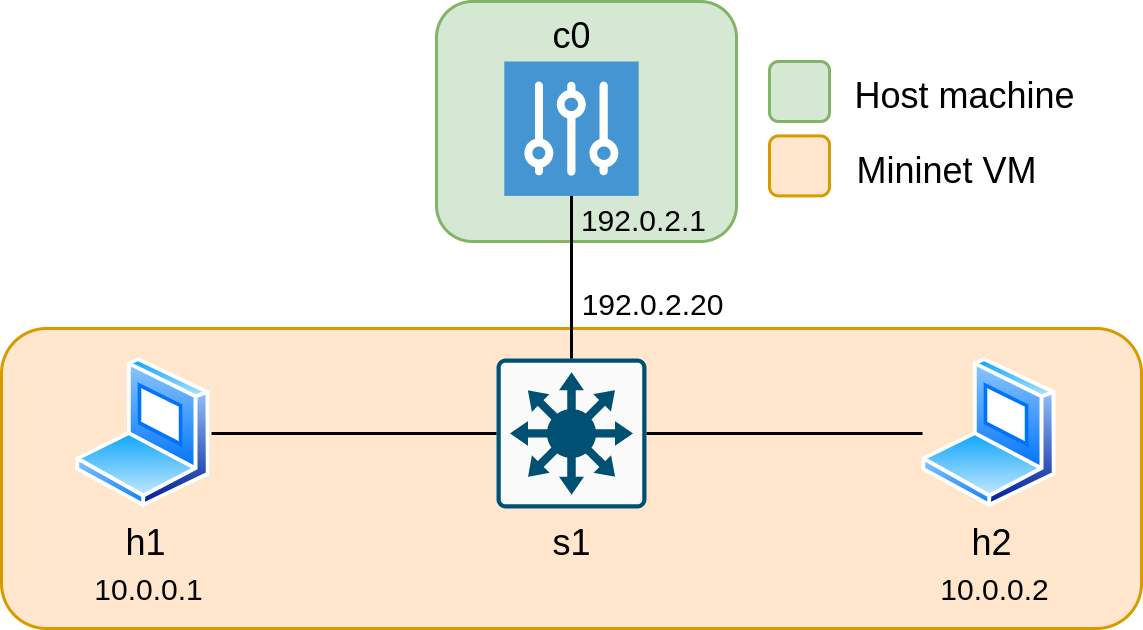
\includegraphics[width=0.6\linewidth]{resources/topology.png}
\end{frame}

\begin{frame}[label=demo-playbook-1]{Demo playbook -- Basic operation}
	\begin{enumerate}
		\item Run the controller
		\item Set up mininet
		\item Start 6 xterm sessions, 3 on each host
		\item Start iperf servers on h1, one for each flow
		\item Run 30Mbps iperf clients, one for each flow
		\item Observe how the default bandwidths ($BW_0$s) are forced
	\end{enumerate}
\end{frame}

\begin{frame}[label=demo-playbook-2]{Demo playbook -- Checking adaptivity}
	\begin{enumerate}
		\item Decrease bandwidth for flow 3 to $10Mbps$
		\item Wait until stats follow the decrease
		\item Observe how other flows can transmit more traffic
		\item Repeat for flow 2 with $BW=6Mbps$
		\item Observe that flow 1 now has $5 + 12.5 + 7.5 = 25Mbps$ assigned
		\item Reset all clients to $30Mbps$ bandwidth
		\item Observe how resources get reassigned
	\end{enumerate}
\end{frame}

\begin{comment}
	Running ONLY f1 being unused with f2 and f3 being used, it won't change
	anything because the portions of the gain are smaller than the hysteresis built
	in the update function.  The minimum step to update is 2 Mbps and the gains for
	each flow would only be 1.25 Mbps.  See
	adapting_monitor_13.py:QoSManager._update_limit()
\end{comment}

\begin{frame}[label=project-limitations]{Project limitations}
	\begin{itemize}
		\item Many parameters are hardwired
		\item Only developed for and tested with UDP flows
		\item Adaptation takes time -- worst case: $50s$
	\end{itemize}
\end{frame}


\section{Screenshots}
\begin{frame}{Full flow use -- terminals}
	\centering
	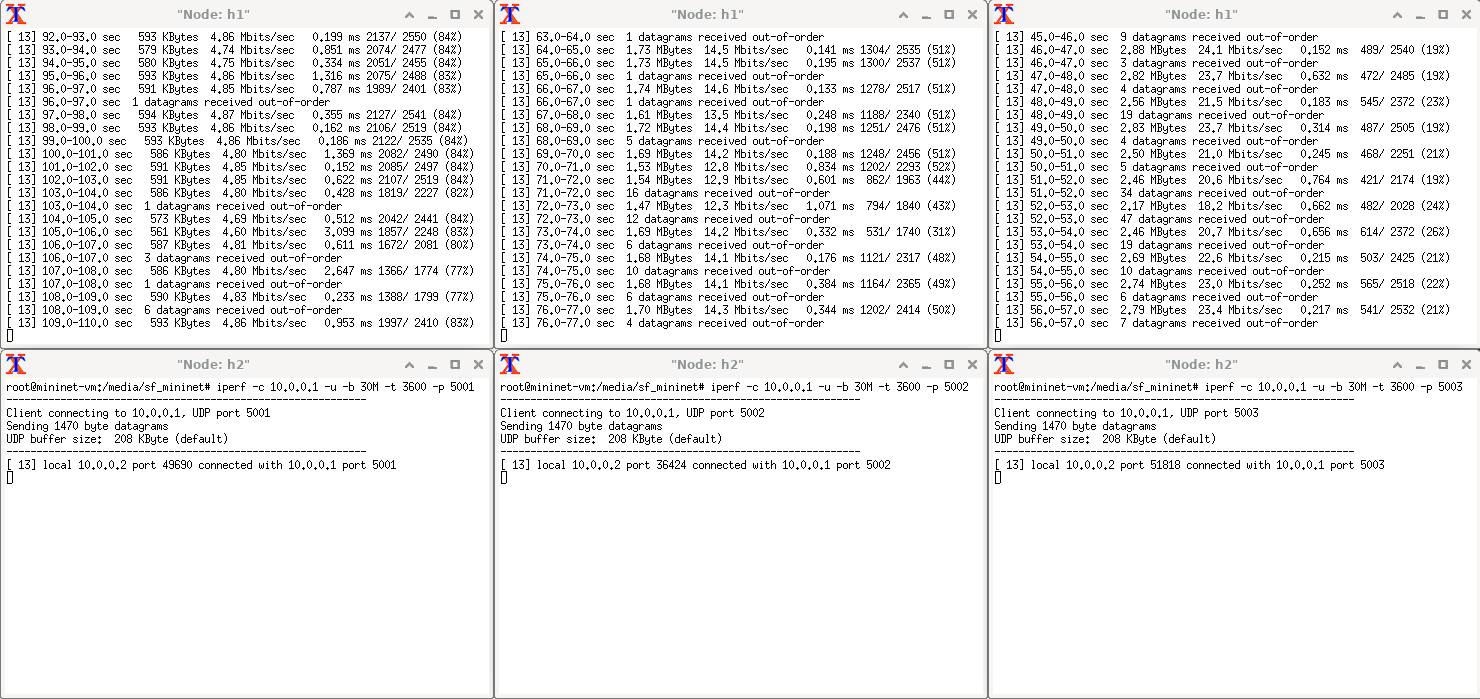
\includegraphics[width=\linewidth]{resources/screenshot-full-use-terminals.png}
\end{frame}
\begin{frame}{Full flow use -- controller stats}
	\centering
	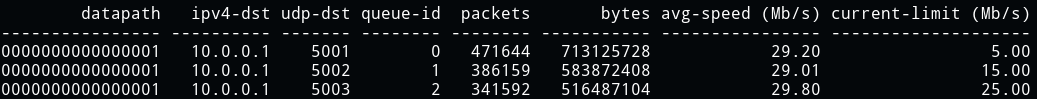
\includegraphics[width=\linewidth]{resources/screenshot-full-use-controllerstats.png}
\end{frame}


\begin{frame}{Flow 3 at 10 Mbps -- terminals}
	\centering
	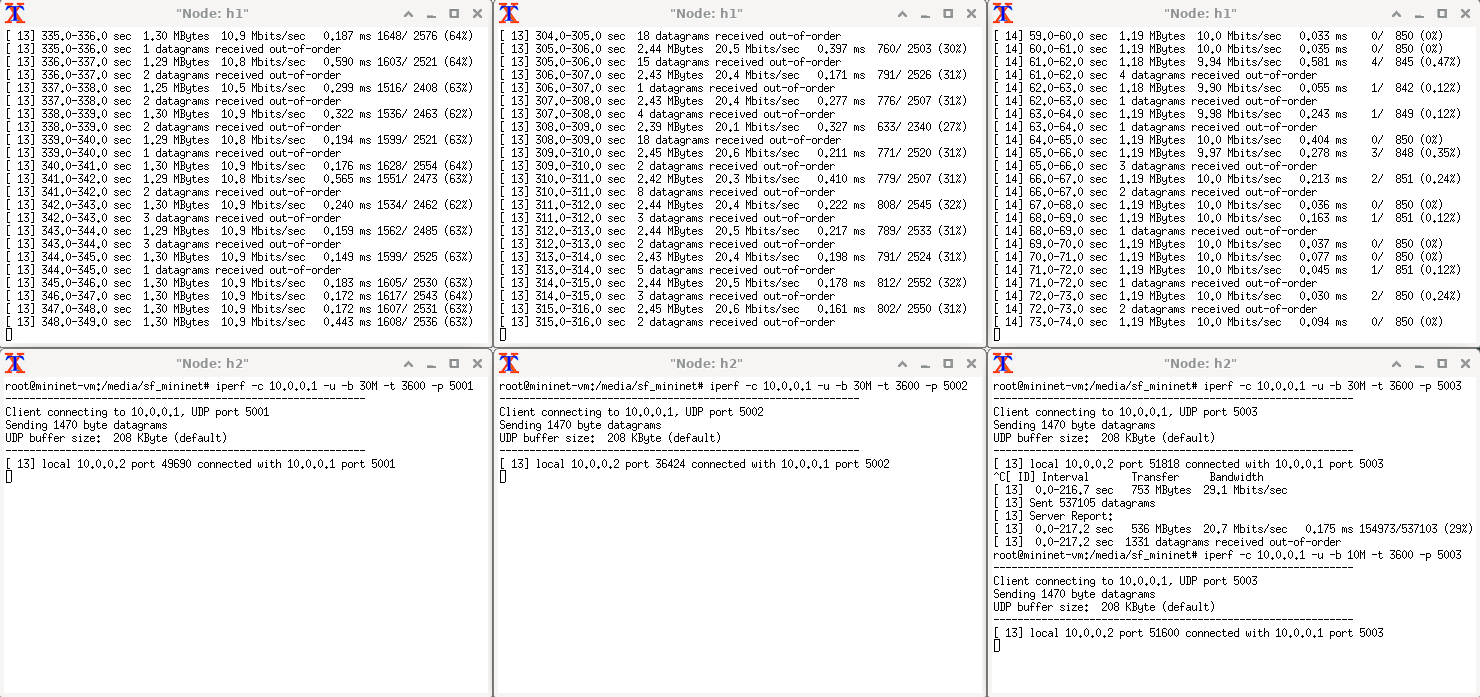
\includegraphics[width=\linewidth]{resources/screenshot-f3-10M-terminals.png}
\end{frame}
\begin{frame}{Flow 3 at 10 Mbps -- controller stats}
\centering
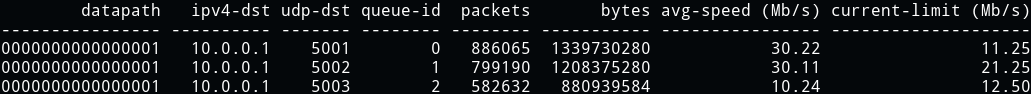
\includegraphics[width=\linewidth]{resources/screenshot-f3-10M-controllerstats.png}
\end{frame}


\begin{frame}{Flow 2 at 6 Mbps -- terminals}
	\centering
	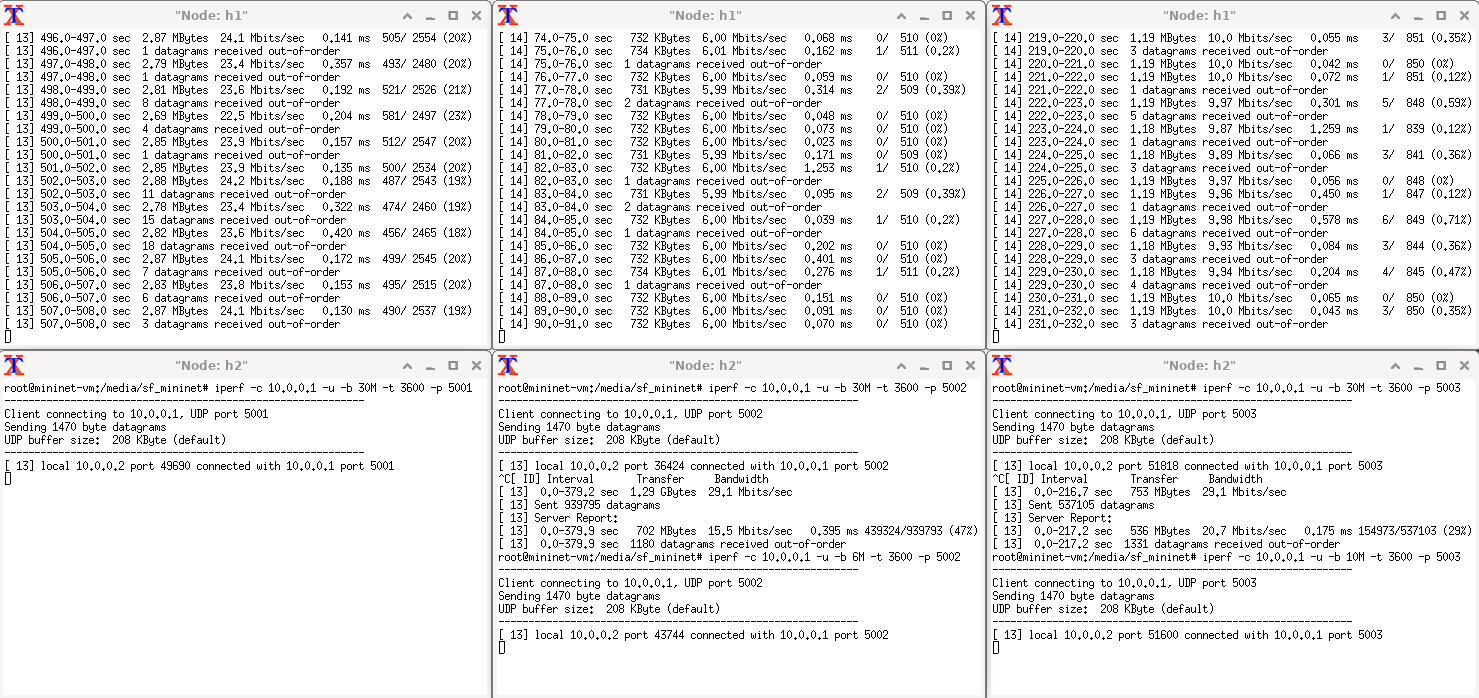
\includegraphics[width=\linewidth]{resources/screenshot-f2-6M-terminals.png}
\end{frame}
\begin{frame}{Flow 3 at 6 Mbps -- controller stats}
	\centering
	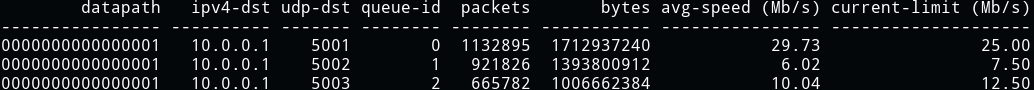
\includegraphics[width=\linewidth]{resources/screenshot-f2-6M-controllerstats.png}
\end{frame}


\begin{comment}
\begin{frame}[allowframebreaks]{References}
	\bibliography{demo.bib}
	\bibliographystyle{IEEEtran}
\end{frame}
\end{comment}
\end{document}
